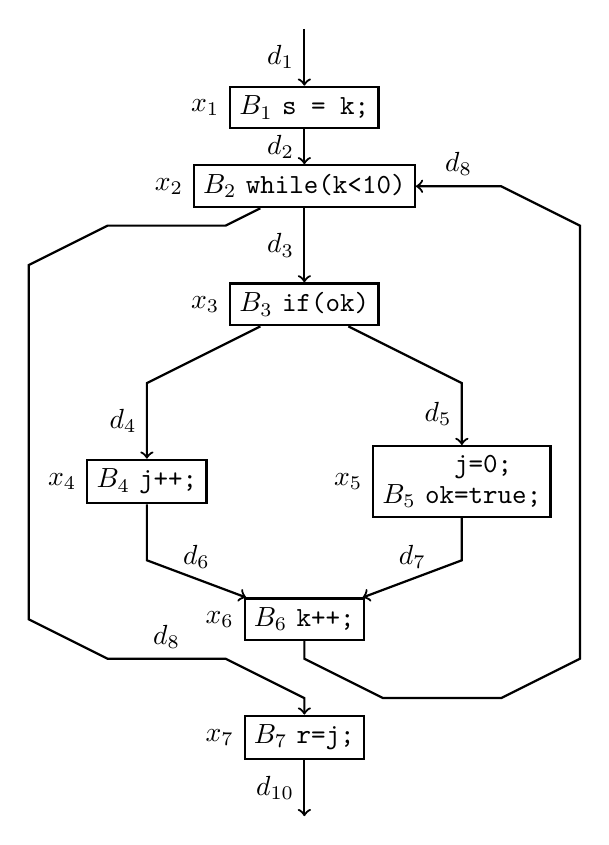
\begin{tikzpicture}	
	\node[rectangle, draw, thick] (n1) at (0, 0) {$B_1$ \texttt{s = k;}};
	\node[rectangle, draw, thick] (n2) at (0, -1) {$B_2$ \texttt{while(k<10)}};
	\node[rectangle, draw, thick] (n3) at (0, -2.5) {$B_3$ \texttt{if(ok)}};
	\node[rectangle, draw, thick] (n4) at (-2, -4.75) {$B_4$ \texttt{j++;}};
	\node[rectangle, draw, thick] (n5) at (2, -4.75) {$B_5$ \shortstack{\texttt{j=0;}\\\texttt{ok=true;}}};
	\node[rectangle, draw, thick] (n6) at (0, -6.5) {$B_6$ \texttt{k++;}};
	\node[rectangle, draw, thick] (n7) at (0, -8) {$B_7$ \texttt{r=j;}};
	
	\node[anchor=east] at (n1.west) {$x_1$};
	\node[anchor=east] at (n2.west) {$x_2$};
	\node[anchor=east] at (n3.west) {$x_3$};
	\node[anchor=east] at (n4.west) {$x_4$};
	\node[anchor=east] at (n5.west) {$x_5$};
	\node[anchor=east] at (n6.west) {$x_6$};
	\node[anchor=east] at (n7.west) {$x_7$};

	\draw[->,thick] (0,1) -- (n1) node[midway,anchor=east] {\texttt{$d_1$}};
	\draw[->,thick] (n1) -- (n2) node[midway,anchor=east] {\texttt{$d_2$}};
	\draw[->,thick] (n2) -- (n3) node[midway,anchor=east] {\texttt{$d_3$}};
	\draw[->,thick] (n3) -- +(-2,-1) -- (n4) node[midway,anchor=east] {\texttt{$d_4$}};
	\draw[->,thick] (n3) -- +(2,-1) -- (n5)node[midway,anchor=east] {\texttt{$d_5$}};
	\draw[->,thick] (n4) -- +(0,-1) -- (n6)node[midway,anchor=south] {\texttt{$d_6$}};
  \draw[->,thick] (n5) -- +(0,-1) -- (n6)node[midway,anchor=south] {\texttt{$d_7$}};
	\draw[->,thick] (n6) -- +(0,-0.5) -- +(1,-1) -- +(2.5,-1) -- +(3.5,-0.5) -- +(3.5,+5) -- +(2.5,+5.5) -- (n2)node[midway,anchor=south] {\texttt{$d_8$}};
	\draw[->,thick] (n2) -- +(-1,-0.5) -- +(-2.5,-0.5) --+(-3.5,-1) -- +(-3.5,-5.5) -- +(-2.5,-6) -- +(-1,-6)node[midway,anchor=south] {\texttt{$d_8$}} -- +(0,-6.5) -- (n7);
  \draw[->,thick] (n7) -- +(0,-1) node[midway,anchor=east] {\texttt{$d_{10}$}};

\end{tikzpicture}